\documentclass[12pt]{article}
\usepackage[top=1in, bottom=1in, right=1in, left=1in]{geometry}
\usepackage{setspace}
\usepackage{graphicx}
\usepackage{setspace}
\usepackage{parskip}
\usepackage{url}

\title{Excepted Appointments and Presidential Unilateral Power}
\date{November 17, 2015}
\author{Emily H. Moore}


\usepackage{Sweave}
\begin{document}
\Sconcordance{concordance:ScheduleCAppointmentsandPresidentialUnilateralPowers.tex:ScheduleCAppointmentsandPresidentialUnilateralPowers.rnw:%
1 13 1 1 0 63 1}

\maketitle
\parindent=0.5in
\parskip=0.01in
\doublespacing

Presidents use a variety of tools to influence both administrative and legislative policymaking. They can experience greater legislative success in Congress by using their veto powers (Cameron 2000) and leveraging bureaucratic expertise (Howell, Jackman, and Rogowski 2013). Presidents may create policy without Congress using executive orders, proclamations, national security directives, and executive agreements (e.g. Howell 2003). They  also possess an extensive array of tools for managing the bureaucracy. They can exploit informational advantages (Gailmard and Patty 2012), regulate strategically (e.g. O'Connell 2008; Yackee and Yackee 2009a, 2009b), and appoint the personnel of their choosing (e.g. Lewis 2008). 

	As Moe (1985) argues, presidents have incentives to use their appointment power to politicize the bureaucracy. Lewis (2008, 2011) shows that presidents bolster this administrative control by increasing the number of appointments available to them, expanding appointment power in key management positions, and strategically placing appointments in agencies with unfavorable politics. Virtually everything we know about the appointment power, however, is based on studies of the very small portion of appointees who undergo Senate confirmation. This is surprising given that the vast majority of bureaucrats are not subject to Senate confirmation but nonetheless perform important functions within the bureaucracy.
	
	To illustrate the importance of excepted appointees, consider the case of Antonio Weiss and the Department of the Treasury. In November 2014, President Obama nominated Weiss, head of investment banking for independent financial management firm Lazard, as the Undersecretary for Domestic Finance. Led by Elizabeth Warren, a number of progressive Democrats in the Senate opposed Weiss' appointment.\footnote{ These Democrats were concerned about Weiss' financial industry ties, believing he may not be willing to produce stringent enough regulations. More information can be found in this article: http://www.politico.com/story/2015/01/antonio-weiss-pulls-out-treasury-undersecretary-114191\\} To avoid a confirmation showdown, Obama withdrew the nomination and instead appointed Weiss as Counselor to the Secretary of the Treasury, a position which does not require Senate confirmation. While he has somewhat less influence as Counselor than he would have as Undersecretary, Weiss had the ability to affect policy immediately rather than undergoing a lengthy battle in the final 2 years of the Obama presidency.	\footnote{ Elizabeth Warren should especially appreciate the importance of these lower-level positions because she served as an excepted Schedule C appointee under Secretary Geithner, appointed for the express purpose of creating the Consumer Financial Protection Bureau.}
	
	This story illustrates two aspects of excepted appointees that make them powerful weapons in the president's unilateral policy arsenal. The first is flexibility. Rather than wait months for appointments to be confirmed and risk potential embarrassment if they are not, presidents can appoint officials who will pursue their agenda immediately. This is especially important given the increasing length of time to confirmation for PAS appointees. The average JFK appointee waited only 2.5 months to be confirmed by the Senate. The average George W. Bush appointee waited nine months, and while Reagan appointed 86 percent of his top officials in his first year, Obama could not complete two-thirds (Pfiffner 2015). Lengthy confirmation ordeals could severely hinder the president's agenda, especially later in a presidency (Lewis 2011; McCarty and Razaghian 1999). Moreover, there may be instances in which positions must be filled quickly in order to fulfill essential tasks in an agency. The second important aspect is ideology. As the Warren-Weiss example shows, presidents can use excepted appointments to appoint individuals that Congress could not or would not confirm. In one instance, Congress may oppose an appointee, leading the president to find other means to hire his preferred candidate. In another, gridlock may prevent Congress from confirming a nominee desirable to a majority of members.
	
	In this paper, I argue that excepted appointees\footnote{As I mention in greater detail in later sections, excepted service appointments are technically those individuals who are not appointed through the competitive hiring process. However, in practice, OPM does not refer to all such employees as excepted. Senate-confirmed appointees carry the distinction``PAS." Most of the excepted service positions to which OPM refers are excepted both from the competitive processes and advice and consent, which is how I choose to use the term.} are relatively invisible, yet consequential tools in the president's unilateral policy arsenal. While excepted appointments lack the glamour and intrigue associated with their PAS counterparts, they are nonetheless responsible for carrying out vital agency tasks. In fact, because these Schedule C appointees are ``invisible" (Lewis and Waterman 2013), they largely fly under the radar of congressional and media oversight, allowing the president to use them with relatively few restrictions. 

		There are a variety of types of excepted appointees ranging in their level of importance and politicization. In this paper, I introduce a dataset of all Schedule C appointments from 1998 to 2014. Examining changes in the number of Schedule C appointments, I show that presidents use these appointments to quickly fill positions for which Senate confirmation would take much longer. I also show that presidents utilize Schedule C appointments to advance their agendas, increasing the number of Schedule C appointees in ideologically distant agencies. In combination, these results show that Schedule C appointees offer the president flexibility and ideological congruence, making them a useful tool in the president's policymaking toolchest.
		
\section*{The Importance of Excepted Appointments}

%%Need to add some more literature on experts v. loyalists controversy.
%%More on politicization
	As a long history of literature suggests, presidents care about how agencies execute policy. Much scholarly work is devoted to the president's tradeoff between competent ``experts" and political loyalists (e.g. Hollibaugh forthcoming; Hollibaugh et al. 2014; Parsneau 2013). While the former cannot necessarily be trusted to advance the president's political interests (Moe 1985), the latter may lack the skill to execute policy well or efficiently (e.g. Lewis 2005; Gilmour and Lewis 2006; Heclo 1975, 1977). A related body of literature explores how the president selects apppointees on competence, ideology, or patronage based on the agency type. (e.g. Hollibaugh et al. 2014; Lewis and Waterman 2013; Patterson 2008; Patterson and Pfiffner 2001; Tolchin and Tolchin 2010). Scholars have been particularly concerned with a tendency for the president to ``politicize" the bureaucracy (that is use appointees selected based on their ties to the party rather than expertise), which many argue is a more recent phenomenon (e.g. Burke 1992; Hart 1995; Heclo 1975; Lewis 2005, 2008; Wayne et al. 1979).
	
Lewis (2008) provides important insights into how presidents politicize. One of the most important results is that presidents focus their politicization efforts on agencies which are ideologically opposed to them. Agency missions tend to differ based on who created them and what they do, and presidents of both parties reach office with bureaus that are naturally in support or opposition. Rather than focus most of their efforts on restaffing agencies which are already inclined to agree with them, they focus instead on molding opposing bureaus. They use higher-level appointees to do this, but they also utilize excepted appointees. Lower level appointees are often responsible for making important policy decisions or carrying out vital agency tasks. Without these lower level appointees, it may be impossible to enact the president's agenda. In an interview, President Ford argued for greater appointment power at the lower levels of the bureaucracy, stating, ``if he [the president] cannot reach into the bowels of a department his decisions way up at the top will seldom be adequately implemented out in the grass roots" (Lewis 2008, 57). Despite their usefulness to the president, lower-level appointees, and especially those who do not face Senate confirmation, are often overlooked in studies.
	
\subsubsection*{Flexbility}
-Need to lead into these sections and then describe literature that suggests flexibility is something the president needs/wants. Ann O'Connell, etc.
\subsection*{Ideology}


\subsection*{Excepted Service and the Larger Appointment System}

	To better study excepted appointments, it is useful to understand how they fit in the appointment system. Most people are familiar with traditional advice and consent appointments. However, most jobs in the bureaucracy are filled through a competitive process open to the public just as industry jobs are filled. A job is posted, people apply for it, there are interviews, and the position is filled. Excepted service positions are technically those appointments that have been excepted from competition via the competitive service. The excepted positions about which we are interested are also excepted from advice and consent, so the president and his office hires these employees without Senate approval. Some excepted service appointments are reserved for positions for which the Office of Personnel Management (OPM) does not or cannot provide a test or standard (professionals such as lawyers are one example). Other excepted service appointments are reserved for those with disabilities or are set aside for interns. These appointments, like competitive service appointments, are largely used to complete the day-to-day operations of the government.	Unlike many other excepted positions, Schedule C appointments are positions excepted for political reasons. OPM describes Schedule C appointments as those positions of a ``confidential" or ``policy-determining nature," for which it is important the employee shares the president's vision for the agency. As an example of their place in real agencies, the Administrator and Deputy Administrator of the EPA are both Senate-confirmed appointees. The EPA's Special Assistant to the Senior Climate Policy Counsel is a Schedule C position as is the White House Liaison. The Chairmen of the Council on Environmental Quality is a PAS appointment while the Special Assistant on Climate Change is a Schedule C appointment. Thus, while the highest positions are Senate-confirmed, they are quickly followed by lower-level, but still important Schedule C appointments. 
	
%%Need to include an image from the plum book here	
	
	President Eisenhower created Schedule C appointments when he first reached office. According to Gailmard and Patty (2012), Eisenhower instituted Schedule C because he was faced with the political realities of being the first Republican to win the presidency in twenty years (leaving him with few trusted advisors) and because the post-World War II era left him with an expansive administrative state, which reached further into the economy and society than had previously been conceived. Schedule C was designed to exist between other classes of appointments---appointees beholden directly to the president, but who did not undergo advice and consent or competitive service processes. Today, Schedule C appointees make up about 15 percent of the president's available appointments in the Plum Book.\footnote{The Plum Book is a government publication released once every four years by Congress. It began in the Eisenhower administration for the same reasons that he created Schedule C: because he did not have enough information about the bureaucracy. The Plum Book lists every appointment available for the president to make.}
	
	Schedule C positions are created uniquely for each employee. When the administration wishes to hire someone via Schedule C, it files papers with OPM detailing the responsibilities of the position to justify a particular pay grade and describes its role within the home agency. When the Schedule C is fired or quits, the position is dissolved. If the administration wishes to hire another person to fulfill the role, it must file the paperwork to create the position anew. In other words, Schedule C appointees are not filling a statutory position; they are filling the administration's current needs.	
	
	Though Schedule C positions are not as prestigious as Senate-confirmed appointments, they can still have an impact on policy. Lewis and Waterman (2013) describe a Department of Justice investigation, which found that a Senior Executive Service and former Schedule C appointee, Monica Goodling, was involved in hiring, firing, and promoting civil servants on the basis of political views. Similar lower level appointees engaged in ``bullying career staff, censoring government reports, and leaking internal documents to outside groups in order to pursue the administration's policy and political goals" (Lewis and Waterman 2013, pg. 36). Lewis and Waterman go on to note of Goodling that despite her ``low" status, she ``initiated a series of crucial, politically and legally questionable decisions" (pg. 36). 
	
%Moving to Data Section	
%	While there are some restrictions, Schedule C appointees have the potential to wield considerable influence and are decidedly political. Figure 1 displays the number of Schedule C appointees from 1998-2013 and the number of Schedule C accessions (new hires and transfers) from 2005-2013. As is visible, the number of accessions in 2009, when Obama takes office, is extraordinarily high---almost matching the total number of appointees in that year. While there is always some turnover during a presidential transition, this turnover is higher for political positions. The number of Schedule C accessions as a percentage of Schedule C employees is typically between 20 and 35 percent. For the Obama transition, the number of accessions as percentage of employees was X percent (REPLACE THIS FOR CURRENT PLOT).

%\begin{figure}[htb]
%\begin{center}
%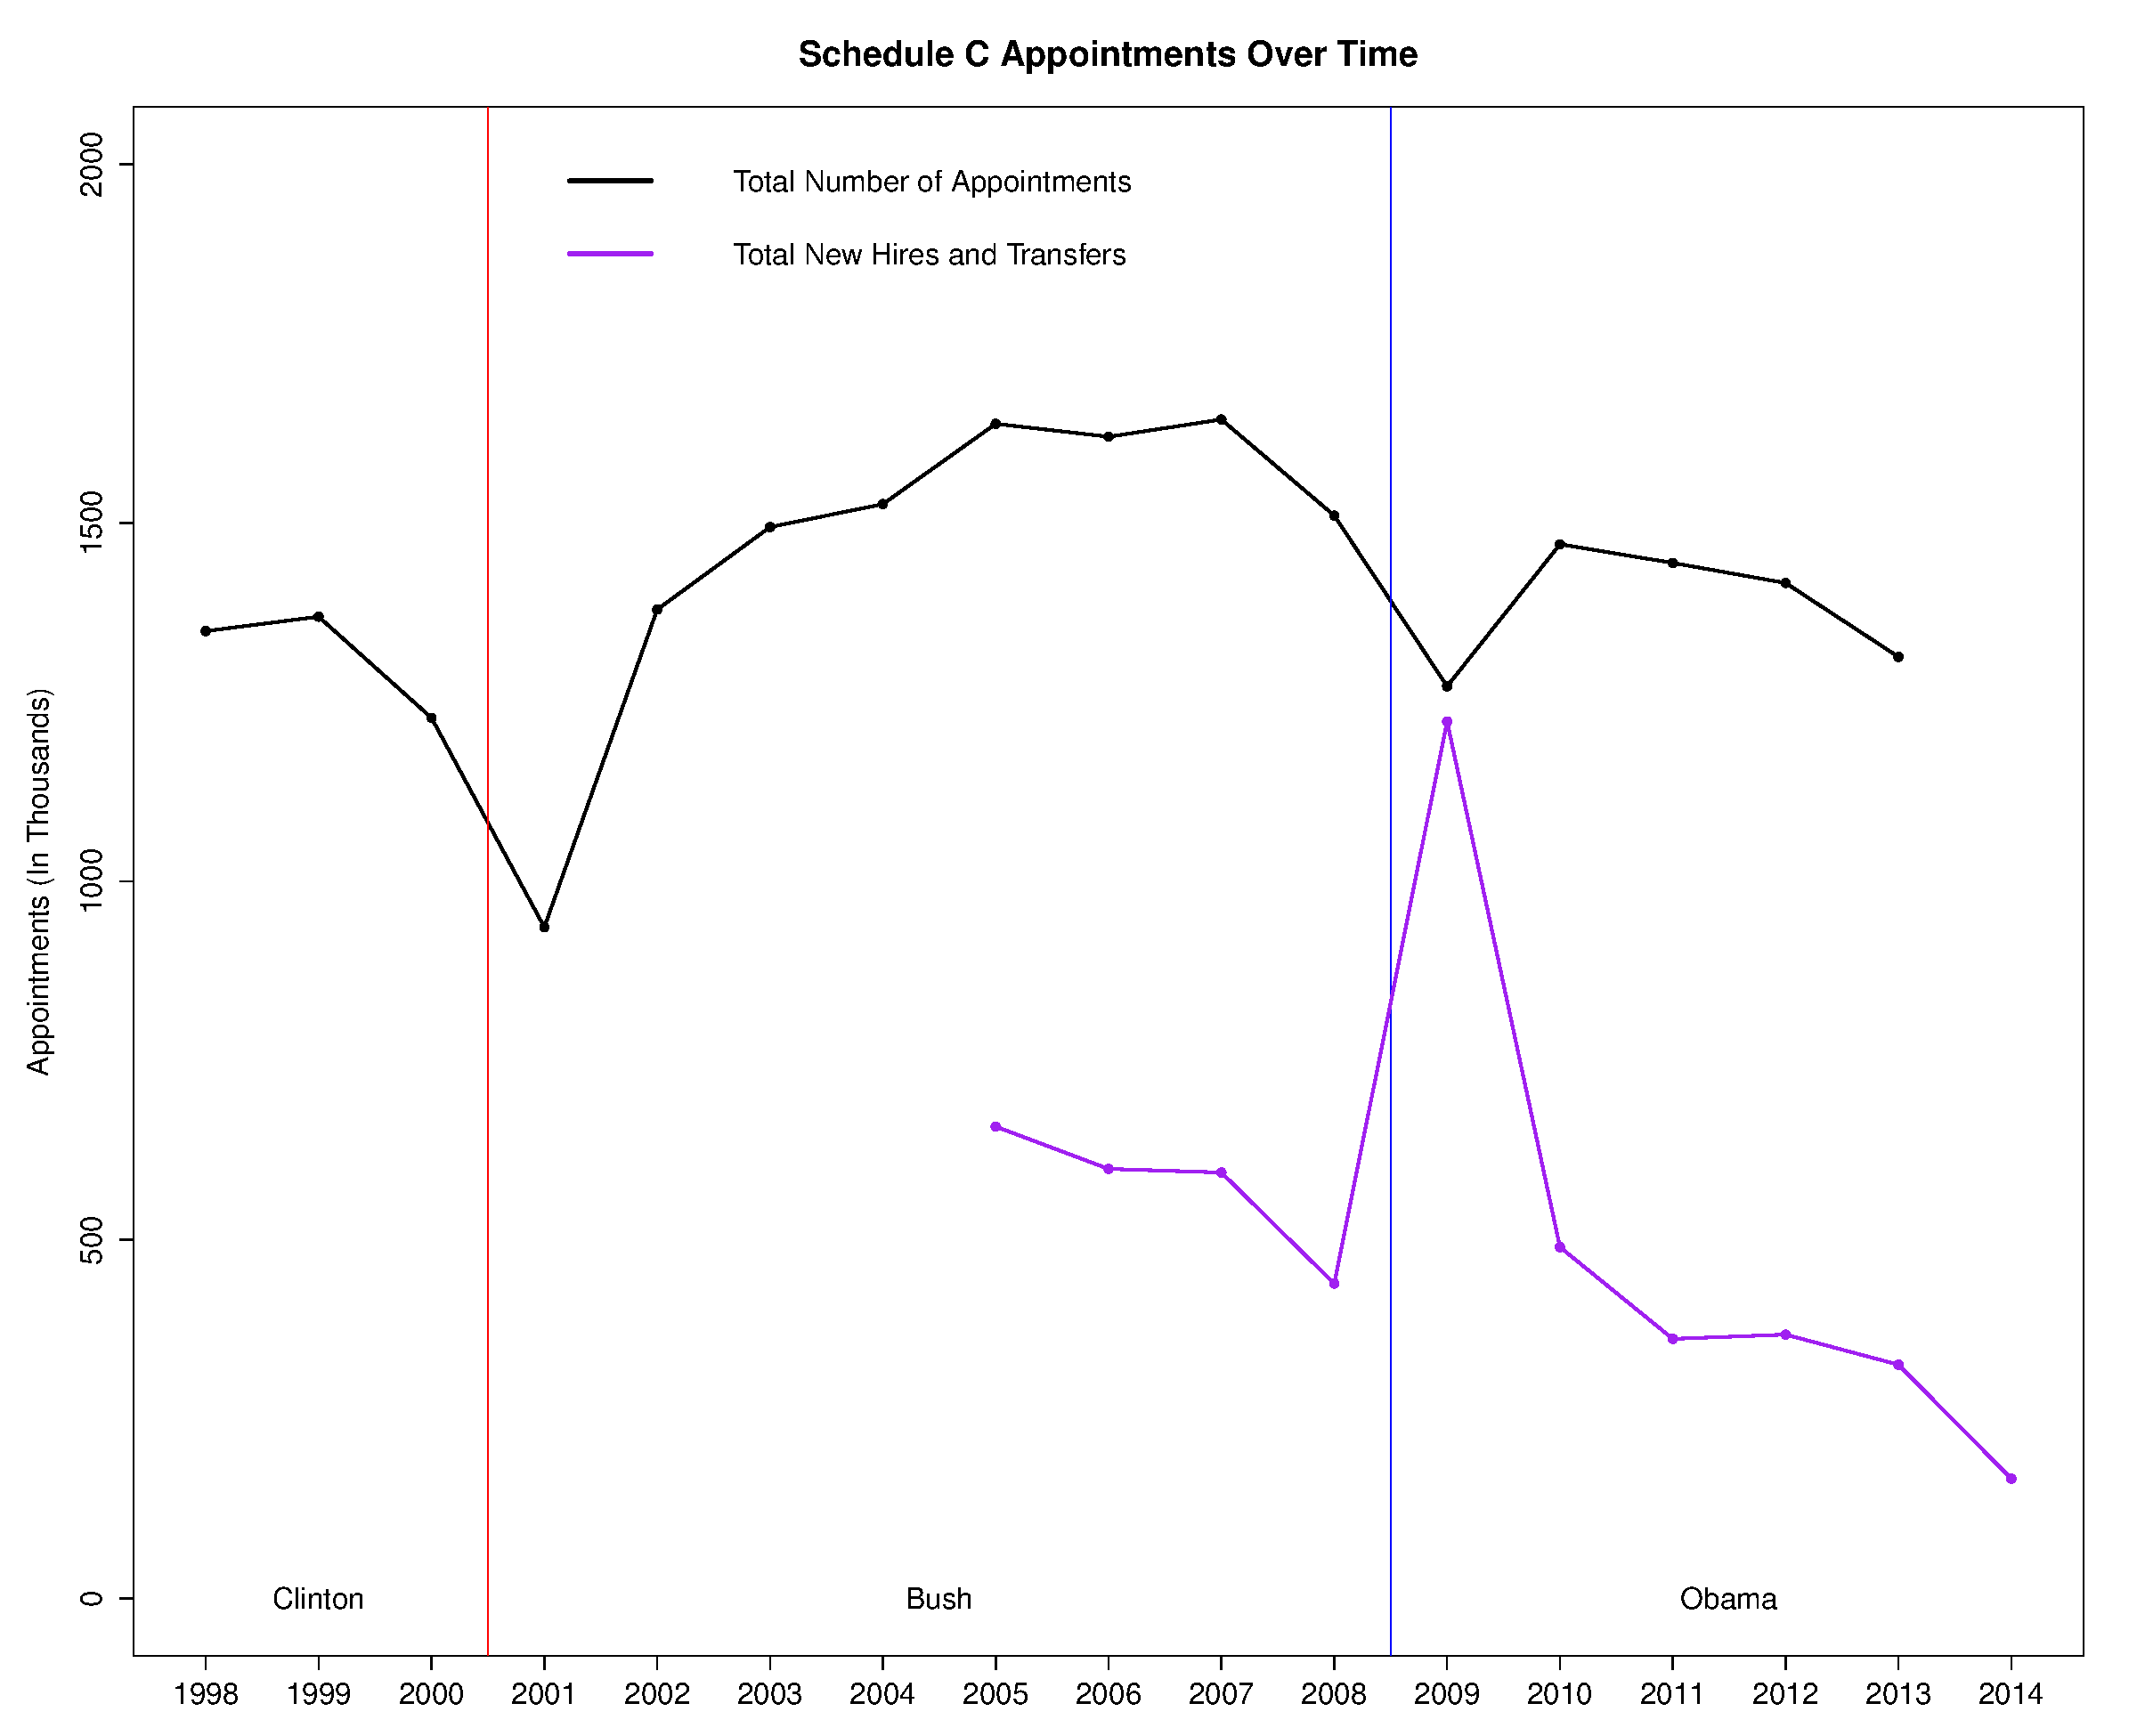
\includegraphics[height=5in,width=6in]{SCAptsandAccOverTime.pdf}
%\caption{Schedule C Appointments Over Time}
%\end{center}
%\end{figure}
	
%Cooney story	
%	If there is any doubt left over the importance of excepted positions, consider the 2005 Cooney scandal in the Council on Environmental Quality (CEQ). The CEQ formulates reports about the status of environmental resources, reviews the environmental activities of governmental and non-governmental organizations, and oversees the implementation of the environmental impact assessment process. While the CEQ is theoretically designed such that environmental experts assess environmental impact, in reality, the process is often political. Phillip Cooney, who served in an excepted position as CEQ Chief of Staff, had only one qualification relating to the job: he had been employed as a lobbyist for the American Petroleum Institute. In 2005, a scandal broke from a report showing that Cooney purposefully doctored expert-prepared government climate reports to downplay scientific climate change findings. One anonymous EPA employee noted that, for many, Cooney's editing had damaged morale and ``created a sense of frustration'' (Revkin 2005a). The Cooney example exemplifies both the importance of excepted appointments as a political tool to advance the president's interests and the power they are able to wield over policies. 

%Miscellaneous sentences to put in other places:
%Many presidents are concerned about the ways in which holdovers from previous administrations might drag their feet or even actively sabotage their agendas. Thus, presidents try to conform agencies to their policy views and they often accomplish this through personnel. 

%It would be easy to conclude that PAS appointees are the only bureaucrats deserving of attention. After all, there is often considerable speculation and controversy surrounding confirmation battles, and these personnel serve in some of the most important positions as cabinet secretaries and heads of independent agencies. 


\end{document}
